%%=============================================================================
%% Methodologie
%%=============================================================================

\chapter{\IfLanguageName{dutch}{Methodologie}{Methodology}}
\label{ch:methodologie}

%% TODO: Hoe ben je te werk gegaan? Verdeel je onderzoek in grote fasen, en
%% licht in elke fase toe welke stappen je gevolgd hebt. Verantwoord waarom je
%% op deze manier te werk gegaan bent. Je moet kunnen aantonen dat je de best
%% mogelijke manier toegepast hebt om een antwoord te vinden op de
%% onderzoeksvraag.

Aan de hand van verchillende RPA providers zal een concreet proces geautomatiseerd worden op Metamaze, het automated document processing platform bij Faktion zelf.


\section{Voorbereiding}
%Ter voorbereiding van het te automatiseren proces bij Faktion heb ik mij eerst ingewerkt op het platform waar dit proces zich voordoet. Ook heb ik de volledige 'RPA Developer Essentials' cursus aangeboden door UiPath gevolgd om een algemene basiskennis rond RPA te beheersen. Daarna is de afweging gemaakt welke RPA software providers nu zullen vergelijken worden. Hieruit zijn 5 kandidaten naar boven gekomen. Als 2 grote providers zal gekeken worden naar UiPath en Automation Anywhere. Voor de kleinere providers wordt gekeken naar AutomationEdge en WorkFusion.

%Ondertussen werd het te automatiseren proces uitgewerkt. Dit proces zal worden geïmplementeerd op de verschillende  platformen. Het gaat hier over het schrijven van een eigen activiteit die in verschillende workflows kan gebruikt worden om te werken met het Metamaze platform.

Eerst en vooral is het MetaMaze platform, gebouwd door Faktion, gronding geëxploreerd geweest. Zo werd een nieuw project aangemaakt, werden er documenten geüpload en gelabeld om een model te kunnen trainen. Nadien werd dit model dan gebruikt om voorspellingen te doen op nieuwe, soortgelijke documenten. Hierbij werd soms expres een verkeerd document geüpload om ook de 'manual intervention' te testen en kijken hoe dit eventueel in een proces kan gegoten worden. Op basis hiervan is een algemeen voorbeeld proces ineen gestoken geweest.

\begin{figure}[h]
	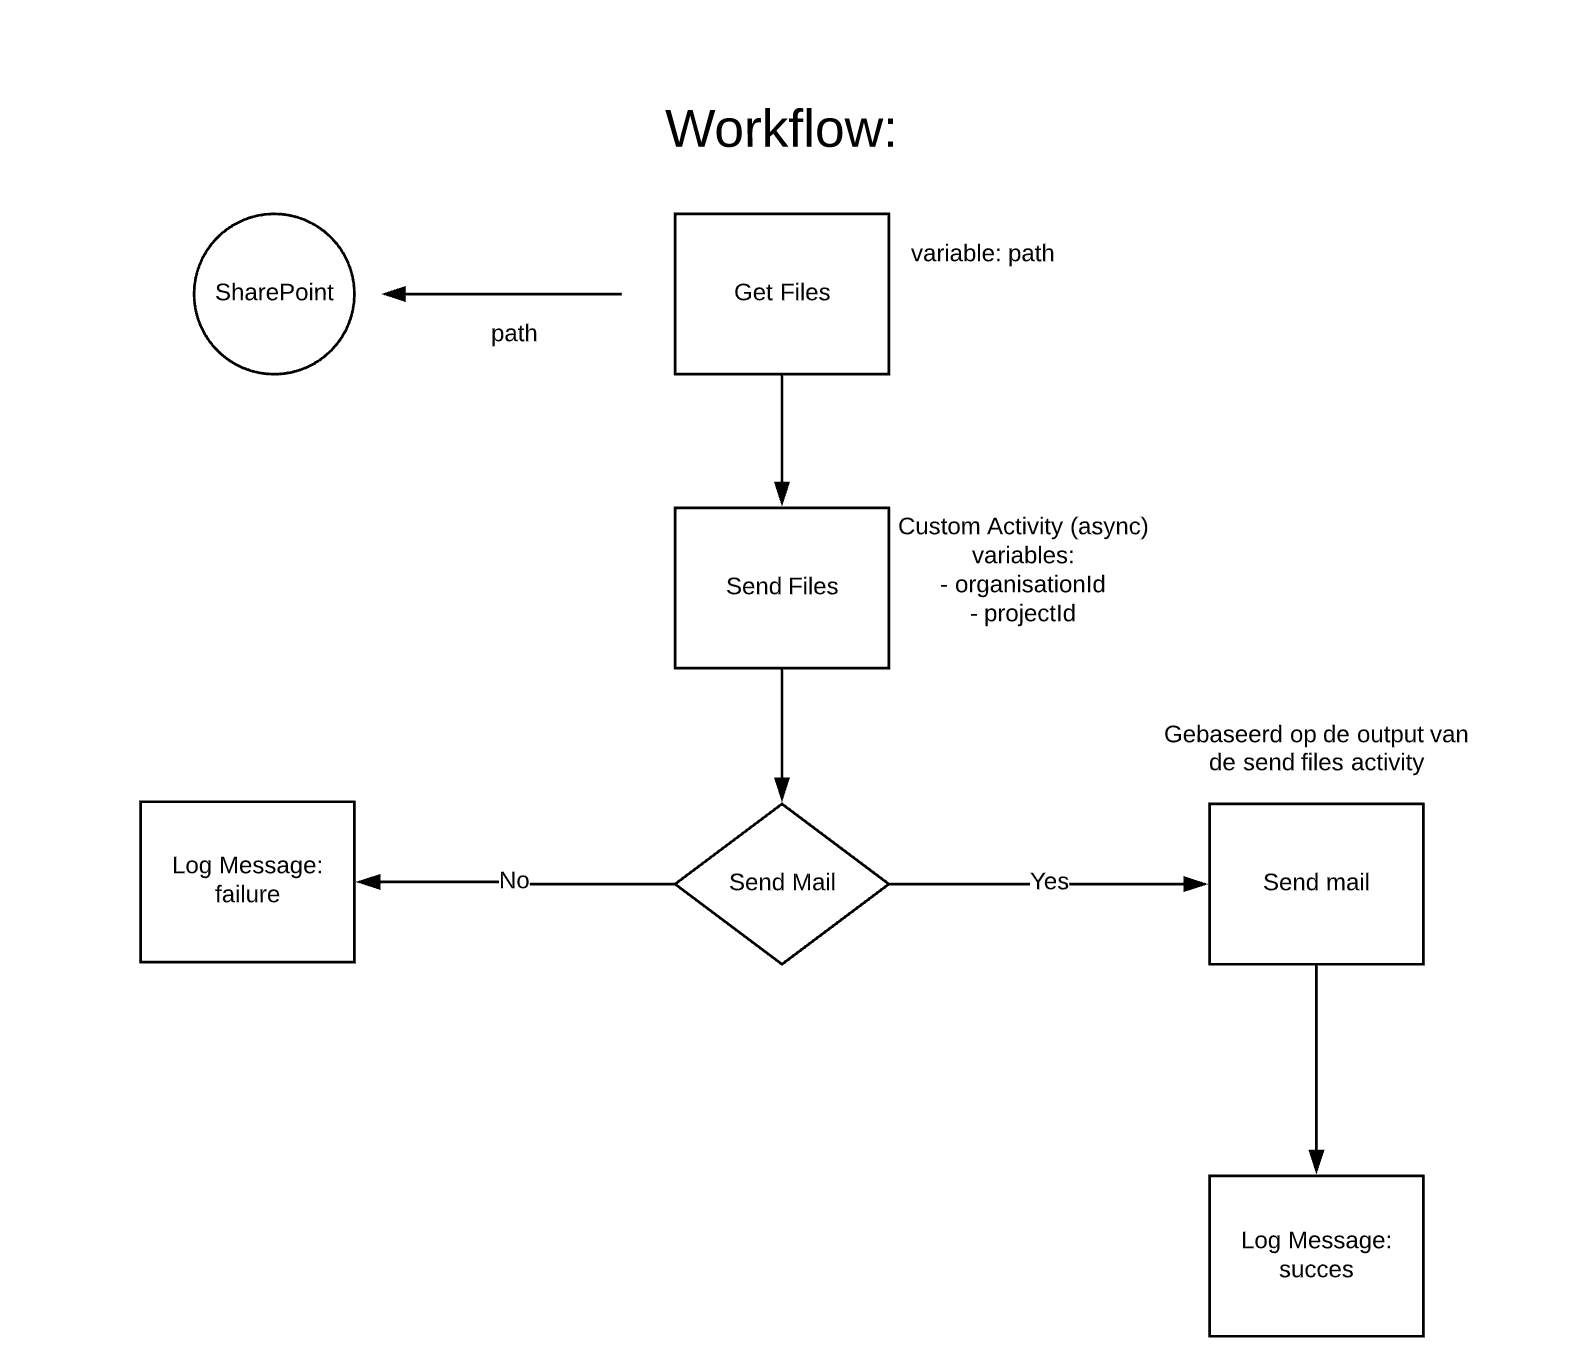
\includegraphics{exampleProcess.png}
	\caption{Voorbeeldproces dat gebruik maakt van de custom Send Files activiteit.}
\end{figure}

Het algemeen proces dat zal geautomatiseerd worden op de verschillende RPA solutions gaat als volgt te werk: Eerst wordt vanuit een bepaald punt (folder op de computer, OneDrive, DropBox, SharePoint) een aantal files opgehaald. Deze files worden doorgegeven aan een zelfgeschreven activiteit. In deze activiteit zullen deze files verstuurd worden naar de MetaMaze API. Nadien wordt er gewacht tot een antwoord terug komt van de server met de resultaten van de upload. Deze resultaten worden terug gegeven naar de volgende stap in de workflow. Door verder te weken met de resulterende JSON kan gekeken worden of de zekerheid waarmee een bepaalde entity dat uit een document is gehaald, onder de minimum zekerheid (threshold) zit of niet. Als er geen onder de threshold zitten wordt het proces afgesloten met een gepaste melding. Als er 1 of meerdere confidence scores onder de threshold zitten zal eerst een mail verstuurd worden naar de klant om te laten weten welke entities de minimum niet gehaald hebben voor dat het proces eindigt met een gepaste melding.

\subsection{Criteria}
De criteria die onderzocht zijn kunnen opgedeeld worden in 3 categorieën: technische criteria, bedrijfscriteria en financiële criteria. Onder de technische criteria valt de mogelijkheid om gemakkelijk zelfgeschreven activiteiten toe te voegen, [...]. Onder bedrijfscriteria vinden we het feit of er een grote onderneming achter het platform staat, hoe actief de community is van het platform, hoe de klantservice is. Tot slot valt onder de financiële categorie natuurlijk de prijs van een enterprise versie maar daarnaast ook of er een mogelijkheid is om een community editie te gebruiken en hoe uitgebreid deze versie is.

De nadruk wordt hier gelegd op een integratie met een eigen API, op een eigen webplatform.

De verschillende criteria hebben elk een zwaarte toegekend gekregen. Hierop worden ze gescoord en op het einde worden alle punten opgeteld.

\subsubsection{Puntenverdeling}
Technische Criteria
\begin{itemize}
	\item custom activities/implementations: /5
	\item implementatietijd: /5
	\item leercurve : /4
\end{itemize}

Bedrijfscriteria
\begin{itemize}
	\item community (forum: hoe actief zijn ze op het forum, ...): /4
	\item klantservice (support, aangeboden cursusen): /4
\end{itemize}

Financiële criteria
\begin{itemize}
	\item prijs (zou niet de bepalende factor mogen zijn): /3
	\item community edition (hoe uitgebreid, representatief?, ...): /5
\end{itemize}


\section{Implementatie}
\subsection{UiPath}
%Gestart met UiPath aangezien ik dit het best kan. Hierbij leek het logisch eerst de custom activity op te bouwen en dan pas alles in een workflow te gieten aangezien de zelfgeschreven activiteit nodig is in de workflow.

%Dit bracht natuurlijk enkele obstakels met zich mee aangezien er wordt gewerkt met de flexibiliteit van de webdev space binnen een strongly typed programmeertaal.

%Eens de custom activity geschreven was lag de enige moeilijkheid nog in het versturen van een mail. Hiervoor werd een standaard SMTP Server gebruikt.

\subsection{Automation Anywhere}
%Al het denkwerk voor het uitwerken van de custom activity was al gebeurd bij UiPath. Het heeft dan ook niet veel tijd gekost om deze om te zetten van een UiPath compatibele activiteit naar een van Automation Anywhere. Het proces zelf uitwerken heeft dan weer wel extra moeite gekost. [...]

\subsection{WorkFusion}
%[...]

\subsection{Intellibot}
\subsection{Microsoft Flow}

\section{Vergelijking}
\begin{table}[h!]
	\centering
	\begin{tabular}{|c||c|c|c|c|c|}
		\hline
		& UiPath & Automation Anywhere & WorkFusion & IntelliBot & Microsoft Flow \\
		\hline
		\hline
		Cursus op het platform & ja     & ja                  & ja         & ja         & nee            \\
		\hline
		Custom Activities& community &  enterprise  & community &  ?         &  ?         \\
		\hline
		Example Row &        &                     &            &            &                \\
		\hline
	\end{tabular}
	\caption{Vergelijking van de verschillende RPA Providers.}
	\label{Vergelijking}
\end{table}
